% Options for packages loaded elsewhere
\PassOptionsToPackage{unicode}{hyperref}
\PassOptionsToPackage{hyphens}{url}
%
\documentclass[
]{article}
\usepackage{lmodern}
\usepackage{amssymb,amsmath}
\usepackage{ifxetex,ifluatex}
\ifnum 0\ifxetex 1\fi\ifluatex 1\fi=0 % if pdftex
  \usepackage[T1]{fontenc}
  \usepackage[utf8]{inputenc}
  \usepackage{textcomp} % provide euro and other symbols
\else % if luatex or xetex
  \usepackage{unicode-math}
  \defaultfontfeatures{Scale=MatchLowercase}
  \defaultfontfeatures[\rmfamily]{Ligatures=TeX,Scale=1}
\fi
% Use upquote if available, for straight quotes in verbatim environments
\IfFileExists{upquote.sty}{\usepackage{upquote}}{}
\IfFileExists{microtype.sty}{% use microtype if available
  \usepackage[]{microtype}
  \UseMicrotypeSet[protrusion]{basicmath} % disable protrusion for tt fonts
}{}
\makeatletter
\@ifundefined{KOMAClassName}{% if non-KOMA class
  \IfFileExists{parskip.sty}{%
    \usepackage{parskip}
  }{% else
    \setlength{\parindent}{0pt}
    \setlength{\parskip}{6pt plus 2pt minus 1pt}}
}{% if KOMA class
  \KOMAoptions{parskip=half}}
\makeatother
\usepackage{xcolor}
\IfFileExists{xurl.sty}{\usepackage{xurl}}{} % add URL line breaks if available
\IfFileExists{bookmark.sty}{\usepackage{bookmark}}{\usepackage{hyperref}}
\hypersetup{
  pdftitle={ISLR Chapter 6 Notes},
  pdfauthor={Ryan Heslin},
  hidelinks,
  pdfcreator={LaTeX via pandoc}}
\urlstyle{same} % disable monospaced font for URLs
\usepackage[margin=1in]{geometry}
\usepackage{color}
\usepackage{fancyvrb}
\newcommand{\VerbBar}{|}
\newcommand{\VERB}{\Verb[commandchars=\\\{\}]}
\DefineVerbatimEnvironment{Highlighting}{Verbatim}{commandchars=\\\{\}}
% Add ',fontsize=\small' for more characters per line
\usepackage{framed}
\definecolor{shadecolor}{RGB}{248,248,248}
\newenvironment{Shaded}{\begin{snugshade}}{\end{snugshade}}
\newcommand{\AlertTok}[1]{\textcolor[rgb]{0.94,0.16,0.16}{#1}}
\newcommand{\AnnotationTok}[1]{\textcolor[rgb]{0.56,0.35,0.01}{\textbf{\textit{#1}}}}
\newcommand{\AttributeTok}[1]{\textcolor[rgb]{0.77,0.63,0.00}{#1}}
\newcommand{\BaseNTok}[1]{\textcolor[rgb]{0.00,0.00,0.81}{#1}}
\newcommand{\BuiltInTok}[1]{#1}
\newcommand{\CharTok}[1]{\textcolor[rgb]{0.31,0.60,0.02}{#1}}
\newcommand{\CommentTok}[1]{\textcolor[rgb]{0.56,0.35,0.01}{\textit{#1}}}
\newcommand{\CommentVarTok}[1]{\textcolor[rgb]{0.56,0.35,0.01}{\textbf{\textit{#1}}}}
\newcommand{\ConstantTok}[1]{\textcolor[rgb]{0.00,0.00,0.00}{#1}}
\newcommand{\ControlFlowTok}[1]{\textcolor[rgb]{0.13,0.29,0.53}{\textbf{#1}}}
\newcommand{\DataTypeTok}[1]{\textcolor[rgb]{0.13,0.29,0.53}{#1}}
\newcommand{\DecValTok}[1]{\textcolor[rgb]{0.00,0.00,0.81}{#1}}
\newcommand{\DocumentationTok}[1]{\textcolor[rgb]{0.56,0.35,0.01}{\textbf{\textit{#1}}}}
\newcommand{\ErrorTok}[1]{\textcolor[rgb]{0.64,0.00,0.00}{\textbf{#1}}}
\newcommand{\ExtensionTok}[1]{#1}
\newcommand{\FloatTok}[1]{\textcolor[rgb]{0.00,0.00,0.81}{#1}}
\newcommand{\FunctionTok}[1]{\textcolor[rgb]{0.00,0.00,0.00}{#1}}
\newcommand{\ImportTok}[1]{#1}
\newcommand{\InformationTok}[1]{\textcolor[rgb]{0.56,0.35,0.01}{\textbf{\textit{#1}}}}
\newcommand{\KeywordTok}[1]{\textcolor[rgb]{0.13,0.29,0.53}{\textbf{#1}}}
\newcommand{\NormalTok}[1]{#1}
\newcommand{\OperatorTok}[1]{\textcolor[rgb]{0.81,0.36,0.00}{\textbf{#1}}}
\newcommand{\OtherTok}[1]{\textcolor[rgb]{0.56,0.35,0.01}{#1}}
\newcommand{\PreprocessorTok}[1]{\textcolor[rgb]{0.56,0.35,0.01}{\textit{#1}}}
\newcommand{\RegionMarkerTok}[1]{#1}
\newcommand{\SpecialCharTok}[1]{\textcolor[rgb]{0.00,0.00,0.00}{#1}}
\newcommand{\SpecialStringTok}[1]{\textcolor[rgb]{0.31,0.60,0.02}{#1}}
\newcommand{\StringTok}[1]{\textcolor[rgb]{0.31,0.60,0.02}{#1}}
\newcommand{\VariableTok}[1]{\textcolor[rgb]{0.00,0.00,0.00}{#1}}
\newcommand{\VerbatimStringTok}[1]{\textcolor[rgb]{0.31,0.60,0.02}{#1}}
\newcommand{\WarningTok}[1]{\textcolor[rgb]{0.56,0.35,0.01}{\textbf{\textit{#1}}}}
\usepackage{graphicx,grffile}
\makeatletter
\def\maxwidth{\ifdim\Gin@nat@width>\linewidth\linewidth\else\Gin@nat@width\fi}
\def\maxheight{\ifdim\Gin@nat@height>\textheight\textheight\else\Gin@nat@height\fi}
\makeatother
% Scale images if necessary, so that they will not overflow the page
% margins by default, and it is still possible to overwrite the defaults
% using explicit options in \includegraphics[width, height, ...]{}
\setkeys{Gin}{width=\maxwidth,height=\maxheight,keepaspectratio}
% Set default figure placement to htbp
\makeatletter
\def\fps@figure{htbp}
\makeatother
\setlength{\emergencystretch}{3em} % prevent overfull lines
\providecommand{\tightlist}{%
  \setlength{\itemsep}{0pt}\setlength{\parskip}{0pt}}
\setcounter{secnumdepth}{-\maxdimen} % remove section numbering

\title{ISLR Chapter 6 Notes}
\author{Ryan Heslin}
\date{11/16/2020}

\begin{document}
\maketitle

\begin{Shaded}
\begin{Highlighting}[]
\KeywordTok{library}\NormalTok{(tidyverse)}
\end{Highlighting}
\end{Shaded}

\begin{verbatim}
## -- Attaching packages --------------------------------------- tidyverse 1.3.0 --
\end{verbatim}

\begin{verbatim}
## v ggplot2 3.3.2     v purrr   0.3.4
## v tibble  3.0.4     v dplyr   1.0.2
## v tidyr   1.1.2     v stringr 1.4.0
## v readr   1.4.0     v forcats 0.5.0
\end{verbatim}

\begin{verbatim}
## -- Conflicts ------------------------------------------ tidyverse_conflicts() --
## x dplyr::filter() masks stats::filter()
## x dplyr::lag()    masks stats::lag()
\end{verbatim}

\begin{Shaded}
\begin{Highlighting}[]
\KeywordTok{library}\NormalTok{(rlang)}
\end{Highlighting}
\end{Shaded}

\begin{verbatim}
## 
## Attaching package: 'rlang'
\end{verbatim}

\begin{verbatim}
## The following objects are masked from 'package:purrr':
## 
##     %@%, as_function, flatten, flatten_chr, flatten_dbl, flatten_int,
##     flatten_lgl, flatten_raw, invoke, list_along, modify, prepend,
##     splice
\end{verbatim}

\hypertarget{rationales-for-rejecting-ols}{%
\subsection{Rationales for Rejecting
OLS}\label{rationales-for-rejecting-ols}}

Several reasons exist to use non-OLS regression:

\begin{enumerate}
\def\labelenumi{\arabic{enumi}.}
\item
  Prediction accuracy. OLS is variant unless \(n >> p\) - there are many
  more observations than predictors. Constraining coefficients will
  reduce bias in this case.
\item
  Interpretability. Models with irrelevant variables are hard to
  interpret; eliminating them simpligies the equation, but OLS almost
  never sets betas at 0.
\end{enumerate}

The three main methods are subset selection, shrinkage, and dimnesion
reduction.

\begin{enumerate}
\def\labelenumi{\arabic{enumi}.}
\item
  What are the three approaches to subset selection? How do tehy differ?
\item
  Why is \(R^2\) an inadequate criterion of model performance?
\item
  What indirect criteria are available to assess test performance?
\item
  What is the rationale for shrinkage methods?
\item
  How do the lasso and ridge regression differ? How may each be viewed
  as an optimization problem?
\item
  How does principal components regression work?
\item
  How are principal components constructed?
\item
  What is the curse of dimensionality?
\end{enumerate}

\hypertarget{subset-selection}{%
\subsection{Subset Selection}\label{subset-selection}}

To truly find the best subset, we would have to fit models for every
proper predictor combination - a prohibitive \(2^p\) models.

The usual algorithm is to fit all possible models with \(k\) predictors
from \(k=1\) to \(k=p\), select a best model for each \(k\) (\(M_{k}\))
by lowest RSS, then select the best \(M_k\) by cross-validated error or
another criterion.

Importantly, RSS and \(R^2\) alone cannot be used to choose the best
\(M_k\), since they always improve as predictors are added. These
statistics tell us only about training error, not test error.

Notice how \(R^2\) increases in the graph.

\begin{Shaded}
\begin{Highlighting}[]
\NormalTok{forms <-}\StringTok{ }\KeywordTok{accumulate}\NormalTok{(}\KeywordTok{colnames}\NormalTok{(mtcars)[}\OperatorTok{-}\DecValTok{1}\NormalTok{], paste, }\DataTypeTok{sep =} \StringTok{" + "}\NormalTok{) }\OperatorTok\StringTok{ }
\StringTok{  }\KeywordTok{map}\NormalTok{(}\OperatorTok{~}\KeywordTok{paste}\NormalTok{(}\StringTok{"mpg ~"}\NormalTok{, .x)) }\OperatorTok\StringTok{ }
\StringTok{  }\KeywordTok{map}\NormalTok{(as.formula) }\OperatorTok\StringTok{ }
\StringTok{  }\KeywordTok{set_names}\NormalTok{(}\KeywordTok{seq_along}\NormalTok{(.))}

\NormalTok{mods <-}\StringTok{ }\KeywordTok{map}\NormalTok{(forms, }\OperatorTok{~}\KeywordTok{lm}\NormalTok{(}\DataTypeTok{data =}\NormalTok{ mtcars, }\DataTypeTok{formula =} \KeywordTok{expr}\NormalTok{(}\OperatorTok{!!}\NormalTok{.x))) }\OperatorTok\StringTok{ }\KeywordTok{map}\NormalTok{(broom}\OperatorTok{::}\NormalTok{glance)}

\KeywordTok{tibble}\NormalTok{( }\DataTypeTok{rsqd =}\NormalTok{ mods }\OperatorTok\StringTok{ }\KeywordTok{map_dbl}\NormalTok{(}\StringTok{"r.squared"}\NormalTok{), }\DataTypeTok{preds =} \KeywordTok{seq_along}\NormalTok{(mods)) }\OperatorTok\StringTok{ }
\StringTok{  }\KeywordTok{ggplot}\NormalTok{(}\KeywordTok{aes}\NormalTok{(}\DataTypeTok{x =}\NormalTok{ preds, }\DataTypeTok{y =}\NormalTok{ rsqd)) }\OperatorTok{+}
\StringTok{  }\KeywordTok{geom_line}\NormalTok{(}\DataTypeTok{col =} \StringTok{"red"}\NormalTok{)}
\end{Highlighting}
\end{Shaded}

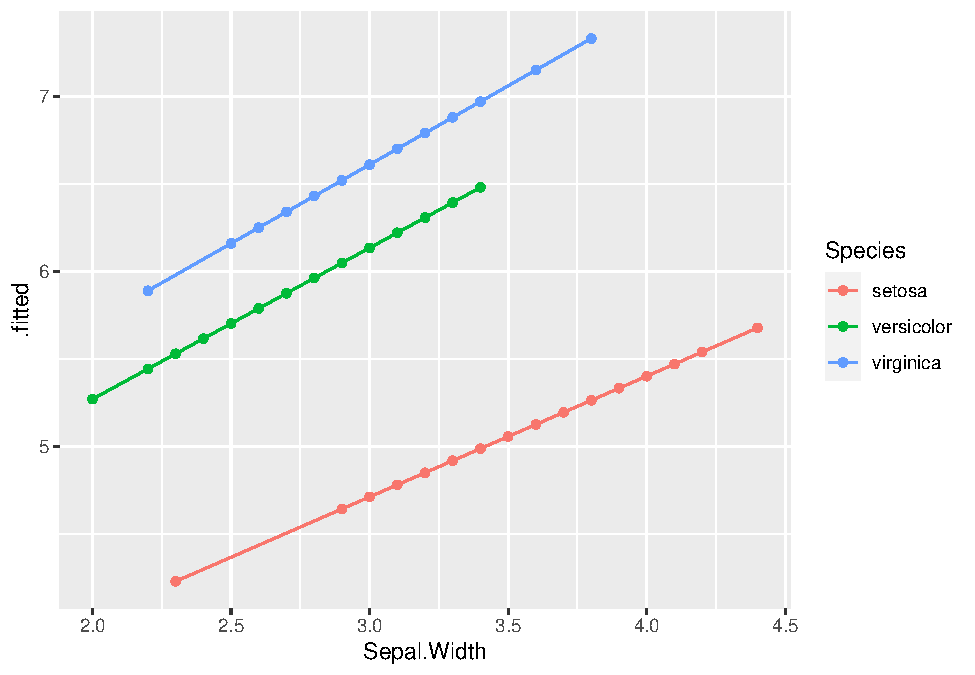
\includegraphics{notes_islr6_files/figure-latex/unnamed-chunk-2-1.pdf}

This kind of subset selection is computationaly expensive and infeasible
past \(p=40\). Many predictors also increases the odds of finding a
model with low test error rate by coincidence.

\hypertarget{forward-stepwise-selection}{%
\subsubsection{Forward Stepwise
Selection}\label{forward-stepwise-selection}}

This apporach starts with the null model, then sequentially adds the
single predictor that best improves the fit until a cutoff point is
reached

\begin{enumerate}
\def\labelenumi{\arabic{enumi}.}
\tightlist
\item
  For \(0 < k <= p\):
\end{enumerate}

\begin{enumerate}
\def\labelenumi{\alph{enumi}.}
\tightlist
\item
  Start with null model \(M_0\)\\
\item
  Fit all \(p-k\) models, each adding a single predictor.
\item
  Choose the best as \(M_{k+1}\)
\item
  Select best \(M_k\) by cross-validation.
\end{enumerate}

This gives a total of just \(\frac{1+p(p+1)}{2}\) models. However, it is
not guaranteed to find the ``best'' model, since each additional
predictor only considers improvement of the previous iteration's model,
locking in the model chosen at the first step; the best model, for
instance, may not contain the predictor that yields the best
single-predictor model.

\hypertarget{backward-stepwise-selection}{%
\subsubsection{Backward Stepwise
Selection}\label{backward-stepwise-selection}}

This approach works in the opposite direction, starting with a full
model and dropping whichever predictor gives the best model when
removed. Unlike forward selection, it requirs \$ n \textgreater p\$
(since the full model cannot have more than \(n\) predictors).

Several hybrid approaches drop variables that give no improvement at
each step.

\hypertarget{choosing-the-best-model}{%
\section{Choosing the Best Model}\label{choosing-the-best-model}}

As noted, RSS and \(R^2\) do not provide meaningful comparisons amond
models with differing numbers of predictors. To get around this, we need
to estimate test error either indirectly or directly.

\hypertarget{indirect-approaches}{%
\subsection{Indirect Approaches}\label{indirect-approaches}}

These techniques adjust training error for model size.

\hypertarget{c_p}{%
\subsubsection{\texorpdfstring{\(C_p\)}{C\_p}}\label{c_p}}

For a model with \(d\) predictors, the equation
\[C_p=\frac{1}{n}(\text{RSS}+2d\hat\sigma^2)\]

where \(\hat\sigma^2\) estimates the error variance of the full (all
predictors) model. This essentially charges the model twice the error
variance for each added predictor. Predictors improve the criterion if
their reduction to RSS outweighs the penalty.

The denominators here essentially represent the expected value of
unexplained variance.

\hypertarget{aic}{%
\subsubsection{AIC}\label{aic}}

The Aikake Information Criterion applies to all models fit by maximum
likelihood, which OLS essentially is. The equation:

\[\text{AIC}=\frac{1}{n\hat\sigma^2}(\text{RSS}+2d\hat\sigma^2)\]

and is just \(C_p\) divided by error variance.

\hypertarget{bic}{%
\subsubsection{BIC}\label{bic}}

The Bayesian information criterion is:

\[\text{BIC}=\frac{1}{n\hat\sigma^2}(\text{RSS}+log(n)d\hat\sigma^2) \]

Since \(log(n) >2\) for any n above 7, the BIC is stricter than \(C_p\)
for models with \(d>7\).

\hypertarget{adjusted-r2}{%
\subsubsection{\texorpdfstring{Adjusted
\(R^2\)}{Adjusted R\^{}2}}\label{adjusted-r2}}

\[\text{Adj. }R^2 = 1 - \frac{\frac{\text{RSS}}{(n-d-1)}}{\frac{\text{TSS}}{(n-1)}})\]

The output of this equation shrinks as predictors are added, so unlike
\(R^2\) bigger values indicate smaller test error. As irrelevant
predictors are added, the RSS in the numerator of the upper subfraction
increases marginally, but is outweighed by the addition of 1 to the
denominator.

\hypertarget{direct-estimation}{%
\subsection{Direct Estimation}\label{direct-estimation}}

Cross-validation and validation sets may be used to simulate test error.
If several models have similar MSE, we pick whichever model within one
SE of the minimum of the error curve has the lowest \(p\).

This graph compares these criteria for several models. It seems clear
that adding the fifth predictor, wt, gives the most improvement.

\begin{Shaded}
\begin{Highlighting}[]
\NormalTok{mods }\OperatorTok\StringTok{ }\KeywordTok{map}\NormalTok{(}\OperatorTok{~}\KeywordTok{select}\NormalTok{(.x, }\KeywordTok{c}\NormalTok{(adj.r.squared, AIC, BIC))) }\OperatorTok\StringTok{ }
\StringTok{  }\KeywordTok{bind_rows}\NormalTok{(}\DataTypeTok{.id =} \StringTok{"Preds"}\NormalTok{) }\OperatorTok\StringTok{ }
\StringTok{  }\KeywordTok{mutate}\NormalTok{(}\DataTypeTok{Preds =} \KeywordTok{as.numeric}\NormalTok{(Preds)) }\OperatorTok\StringTok{ }
\StringTok{  }\KeywordTok{pivot_longer}\NormalTok{(}\OperatorTok{-}\NormalTok{Preds, }\DataTypeTok{names_to =} \StringTok{"Stat"}\NormalTok{) }\OperatorTok\StringTok{ }
\StringTok{  }\KeywordTok{ggplot}\NormalTok{(}\KeywordTok{aes}\NormalTok{(}\DataTypeTok{x =}\NormalTok{ Preds, }\DataTypeTok{y =}\NormalTok{ value, }\DataTypeTok{col =}\NormalTok{ Stat)) }\OperatorTok{+}
\StringTok{  }\KeywordTok{geom_point}\NormalTok{()}\OperatorTok{+}
\StringTok{  }\KeywordTok{geom_line}\NormalTok{()}\OperatorTok{+}
\StringTok{  }\KeywordTok{facet_wrap}\NormalTok{(Stat }\OperatorTok{~}\StringTok{ }\NormalTok{., }\DataTypeTok{scales =} \StringTok{"free_y"}\NormalTok{) }\OperatorTok{+}
\StringTok{  }\KeywordTok{labs}\NormalTok{(}\DataTypeTok{title =} \StringTok{"Models on mtcars"}\NormalTok{)}
\end{Highlighting}
\end{Shaded}

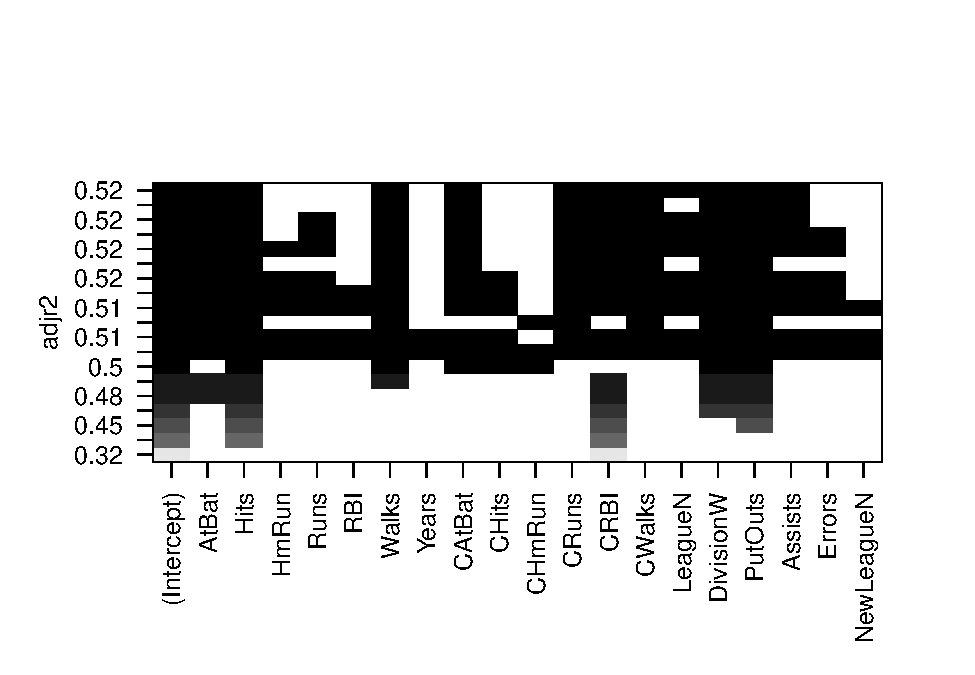
\includegraphics{notes_islr6_files/figure-latex/unnamed-chunk-3-1.pdf}

\hypertarget{shrinkage-methods}{%
\section{Shrinkage Methods}\label{shrinkage-methods}}

Instead of individually dropping or adding predictors, we could fit all
of them but shrink some coefs to 0 or near 0, effectively dropping them.
Shrinking coefficient estimates reduces variance, which is high when
there are many predictors.

\hypertarget{ridge-regression}{%
\subsection{Ridge Regression}\label{ridge-regression}}

You remember, surely, that

\[\text{RSS}=\sum^n_{i=1}(y_i-\beta_0-\sum^p_{j=1}\beta_jx_i)^2\]

Ridge regression adds a minimization constraint to the RSS formula, to
wit:

\[\text{RSS}=\sum^n_{i=1}(y_i-\beta_0-\sum^p_{j=1}\beta_jx_i)^2 +\lambda\sum^p_{j=1}\beta^2_i\]

\(\lambda\) is a tuning parameter that scales the sum of squared beta
coefficients. The closer the betas are to 0, the less they increase this
term. The betas approach but never reach 0 (except if \(\lambda\) is
infinite) because they still need to be nonzero to minimize RSS. Higher
values of lambda steepen the penalty, reducing beta estimates toward
zero. The estiamted vetas vary for each \(\lambda\). Note we don't care
about shrinking \(\beta_0\), since this represents the mean of the
response where all \(x_i=\overline{x}_i\) (or 0, if the data are
mean-centered) and has no realtionship to the assoication of the
response and predictors.

As \(\lambda\) increases, the values of coeffcients tend to devrease at
differnt rates, though individual betas may increase over some ranges of
\(\lambda\). Increasing lambda also lowers the l2 norm of the betas (or
the magnitude - the sqaure root of the summed sqaures, idnicating
distance from 0).

An important caution: standard OLS betas are scale equvariant:
multiplying \(X\) by \(C\) just scales each by \(1/C\). This does not
apply to ridge regression, since the sqauring of the betas breaks the
linear relationship. Ridge regression should therefore \emph{never be
done without standardizing}.

\hypertarget{how-ridge-regression-improves-ols}{%
\subsubsection{How Ridge Regression Improves
OLS}\label{how-ridge-regression-improves-ols}}

AS \(\lambda\) rises, the fit becomes less flexible, reducing variance
at the expense of bias. FOr a model with many predictors, reducing the
variance reduction is welcome. For values of \(\lambda\) up to about 10,
the biad increase is trivial, leading to a substantial reduction in MSE
before increasing bias worsens the fit. In linear relationships, OLS
estiamtes tend to have low bias but high variance (i.e., high likley
test error), especally with many predictors. Ridge regression is also
computationally cheap.

\hypertarget{the-lasso}{%
\subsection{The Lasso}\label{the-lasso}}

Ridge regression does not actually drop any preidctors unless
\(\lambda\) is infinite, leading to models with excess variables. The
lasso minimizes:

\[\text{RSS}+\lambda\sum^p_{j=1}\mid\beta_j\mid\]

so the scaled sum is of the absolute values of the betas rather than the
squares. This gives the l1 norm of the beta vector - the sum of the
magnitudes of the vector's components, or the taxicab distance. This
causes the lasso to select variables, zeroing the betas for high enough
values of \(\lambda\). As \(lambda\) rises, predictors are added and
dropped unpredictably, and the final model may include any number of
them

\hypertarget{alternate-view-of-the-lasso-and-ridge-regression}{%
\subsection{Alternate View of the Lasso and Ridge
Regression}\label{alternate-view-of-the-lasso-and-ridge-regression}}

These methods may be viewed as linear programming problems, wehre RSS is
minimzed subject to the lambda term. In other words, on a p-dimensional
sysetm where each beta defines an axis, where does the region
demarcating a certain quantity of RSS touch the constriant region? The
sum \(s\) of squared betas (or absolute values, for the lasso) may be
viewed as a budget constraining the estiamtion of the coefficients. For
each value of \(\lambda\), \(s\) represents a condition on the betas
estiamted by OLS. That budget is uuique for each value of \(\lambda\).
The larger the coefficient estiamtes, the higher this budget.
Geometrically, the problem involves finding the point where the contours
of the RSS region (ellipses surrounding the point of minimum RSS,
increasing in area as RSS increases) touch the constraint region (a
diamond for the lasso and a circle for ridge regression).These shapes
arise from the differing penalization functions: a linear combination of
the betas for the lasso, a linear combination of squares of betas for
ridge regression The shapes are of course more complex if there are more
predictors.

\[\text{minimize RSS subject to}\sum^p_{j=1}\mid\beta_j\mid <= s\]

In the case of best subset selection, the constraint is:

\[ \sum^p_{j=1}I(\beta_j !=0) <= s \] i.e., no more than \(s\)
predictors can be used. The value of \(s\) and the RSS mminimizers are
linked; neither precedes the other, and solving the problem involves
finding the point of overlap.

If the area of the constriant function overlaps with minimum of RSS,
then a standard OLS estiamte solves the problem. If not, the lambda
estimate is chosen that corresponds to the smallest RSS that touches the
area of the constraint function. This is why the lasso can zero out
predictors; the absolute value function that gives the area of the
constraint has vertices on the axes, so one or more coefficients will
equal zero if the RSS region touches that point.

\hypertarget{comparing-rr-and-the-lasso}{%
\subsubsection{Comparing RR and the
Lasso}\label{comparing-rr-and-the-lasso}}

Ridge regression does better if all predictors are related to the
response, even marginally, since every true \(/beta\) will be nonzero.
Where many predictors are irrelevant, the lasso does better.
Cross-validaton can be used to ascertain which scenario matches the
data.

\hypertarget{the-bayesian-view-of-rr-and-the-lasso}{%
\subsubsection{The Bayesian View of RR and the
LAsso}\label{the-bayesian-view-of-rr-and-the-lasso}}

From the Bayesian persepctive, the coef vector \(\beta\) has an unknown
prior distribution. Menawhile, the data has a likelihood distribution
\[f(Y\mid{X}, \beta)\], where each observed predictor is its own vector.
Multiplying these two gives the posterior distribution:

\[f(Y\mid{X}, \beta)p(\beta)\] , assuming \(X\) is fixed. Assume further
that \[p(\beta)=\prod^p_{j=1}g(\beta_j)\], where \(g\) is a density
function. RR and the lasso correspond to two special cases of this model
(making the usual LM assumption of normally distributed residuals):

\begin{enumerate}
\def\labelenumi{\arabic{enumi}.}
\item
  If \(g\) is noramlly distriubted with mean zero and \(\sigma\) a
  function of \(\lambda\), ridge regression gives the posterior mode
  (the most likely value) of \(\beta\).
\item
  If \(g\) is a double exponential (Laplace) distribution with mean zero
  and a scale parameter a function of \(\lambda\), then the lasso is the
  posterior mode of \(\beta\), though not the posterior mean. This is a
  sharply peaked distribution, consistent with many \(\beta\)s being
  zero.
\end{enumerate}

This aligns with the form of each method - RR modifies the coefs by a
proportion, the lasso by a constant value.

\hypertarget{illustration-a-simple-case}{%
\subsubsection{Illustration: A Simple
Case}\label{illustration-a-simple-case}}

Say that \(n=p\) and X is the identity matrix. Assume also we are
ignoring the intercept, so the optimal solution is:

\[\beta_i=y_i\]

Here, the ridge regression estimate is:
\[\beta_j=\frac{y_i}{1+\lambda}\]

while the lasso adds to \(y_i\) \(\frac{\lambda}{2}\) if
\(y_i > \frac{\lambda}{2}\), adds it if y\_i \textgreater{}
\(y_i < -\frac{\lambda}{2}\), and zeroes betas whose absolute value is
less than \(\frac{\lambda}{2}\). In other words, ridge regression
shrinks coefficients by a proportion, the lasso by a constant.

\hypertarget{selecting-the-tuning-parameter}{%
\subsubsection{Selecting the Tuning
Parameter}\label{selecting-the-tuning-parameter}}

This is typically done by cross-validation, selecting whichever
\(\lambda\) has the smallest error.

\hypertarget{dimension-reduction-methods}{%
\section{Dimension Reduction
Methods}\label{dimension-reduction-methods}}

An alternate solution to many predictors is to transform them into a
smaller number of objetcs. We do this by creating \(M <p\) linear
combination of the predictors.

\[Z_m=\sum^p_{j=1}\phi_{jm}X_j\]

with constants \(\phi\). Remember each \(X\) here is an \(n\)-length
vector; multiplying the \(n\times{p}\) data matrix by every eigenvector
will create an \(n\times{p}\) matrix. Note that there is a separate
\(\phi\) for each predictor for each \(M\) of the transformed variables
(e.g., the \(p \times m\) loadings matrix in factanal). The model then
becomes:

\[y_i = \theta_0 + \sum^M_{m=1}\theta_mz_{im}+\epsilon_i\]

where each \(\theta_m\) is the regression weight and each \(z_{im}\) is
an element of one of the \(M\) vectors of transformed values (e.g., a
single factor). This is simply OLS useing transforemd values of the
predictors.

It follows that
\[\sum^M_{m=1}\theta_mz_{im} =\sum^M_{j=1}\theta_m\sum^p_{j=1}\phi_{jm}x_ij =\sum^p_{j=1}\sum^M_{j=1}\theta_m\phi_{jm}x_{ij}=\sum^p_{j=1}\beta_jx_{ij}\]

so each predictor's beta is the sum of each component's regression
weight multiplied by the constant \(\phi_j\) for that predictor for that
component. \[\beta_j=\sum^M_{m=1}\theta_m\phi_{jm}\]This is thus a
special case of linear regression. In all cases, the predictors are
transformed, and then the model is fitted.

\hypertarget{principal-components-overview}{%
\subsection{Principal Components
Overview}\label{principal-components-overview}}

Yes, the square root of an eigenvalue represents a component's standard
deviation. This is why components with higher eigenvalues capture more
variance: the projected data points are spread further along the
component.

In PCA, the first principal component (an \(m\times{n}\) components
matrix formed by multiplying the transpose of \(m\) eigenvectors by
transposed, scaled data) represents the direction of most variation.
Projecting observations onto these lines would capture maximum variance.
This amounts to translating the greatest shares of variances \(X\) into
scalar coordinates on the components. It might turn out to be:

\[Z_1 = .839\times(pop - \bar{pop}) + .544\times(ad - \bar{ad})\]

where the coeffictents are the loadings \(\phi_{11}\) and \(\phi_{12}\)
of the two predictors - the constants by which the raw scores are
multiplied to transform the data. For each component, the loadings are
the values of the corresponding eigenvector (reading downwards).
Remember in PCA the components are linear combinations of the
predictors. Each \(z_{in}\) is a principal component score. In factanal,
we find these scores and then reconstruct the predictors from them.

Scaling should be done, becuase PCR is sensitive to units of measure.

The first PC is equivalently the direction of maximum variance (i.e.,
the line on which the data would be spread farthest apart if projected)
or the line that minimizes summed distances from the data to the line -
this is what is meant by ``capturing'' variance. It turns out these two
criteria give the same result. These lines are eigenvectors because
eigenvectors represent the direction a transforming matrix ``points''
vectors when used to project them; they satisfy \(Av =\lambda{v}\),
meaning the eigenvector is \emph{not} distorted by the matrix, only
scaled. Each eigenvector corresponds to the matrix's distorting effect
in one dimension. Since they are derived from the correlation (or
covaraince) matrix, which translatest he data vectors to a a coordinate
system that expresses their relationships
(\(\frac{X^T}{\sigma_{X}}\frac{X}{\sigma_{X}}\times \frac{1}{n}\)),
eigenvectors represent directions of maximum variance. Projecting points
onto the PC - achieved by multiplying by the loadings - thus maximizes
their spread along the PC line. Subsequent components must be
uncorrelated (orthogonal; i.e., dot product of zero) in order to capture
remaining variance. The regression is fitted using the transformed
components as x-values.

This plot shows how eigenvectors retain their position after a matrix
transformation. Since the correlation is inverse, the main axis is
negative. \emph{Eigenvectors for a symmetric real matrix are orthogonal
(dot product 0)}.

The eigenvectors of this two-dimensional matrix have elements of
absolute value about .7017, which corresponds ot 45 degrees on the unit
circle.They are othogonal.

\begin{Shaded}
\begin{Highlighting}[]
\NormalTok{dat <-}\StringTok{ }\NormalTok{mtcars }\OperatorTok\StringTok{ }\KeywordTok{select}\NormalTok{(wt, mpg) }\OperatorTok\StringTok{ }
\StringTok{  }\KeywordTok{cor}\NormalTok{()}
\NormalTok{eigens <-}\StringTok{ }\NormalTok{dat }\OperatorTok\StringTok{ }\KeywordTok{eigen}\NormalTok{()}
  
\NormalTok{dat <-}\StringTok{ }\NormalTok{dat }\OperatorTok\StringTok{ }\KeywordTok{as.matrix}\NormalTok{() }\OperatorTok
\StringTok{  }\KeywordTok{as.data.frame}\NormalTok{() }\OperatorTok
\StringTok{  }\CommentTok{# rownames_to_column() %>% }
\StringTok{  }\CommentTok{# pivot_longer(c(wt, mpg)) %>% }
\StringTok{  }\CommentTok{# unite(rowname, name, col = "name") %>% }
\StringTok{  }\KeywordTok{cbind}\NormalTok{(}\KeywordTok{t}\NormalTok{(eigens}\OperatorTok{$}\NormalTok{vectors))}

\KeywordTok{ggplot}\NormalTok{(}\DataTypeTok{data =}\NormalTok{ dat, }\KeywordTok{aes}\NormalTok{(}\DataTypeTok{x =}\NormalTok{ wt, }\DataTypeTok{y =}\NormalTok{ mpg)) }\OperatorTok{+}
\StringTok{  }\KeywordTok{geom_point}\NormalTok{() }\OperatorTok{+}
\StringTok{  }\KeywordTok{geom_segment}\NormalTok{(}\KeywordTok{aes}\NormalTok{(}\DataTypeTok{xend =} \DecValTok{0}\NormalTok{, }\DataTypeTok{yend =} \DecValTok{0}\NormalTok{))}\OperatorTok{+}
\StringTok{  }\KeywordTok{geom_point}\NormalTok{(}\KeywordTok{aes}\NormalTok{(}\DataTypeTok{x =} \StringTok{`}\DataTypeTok{1}\StringTok{`}\NormalTok{, }\DataTypeTok{y =} \StringTok{`}\DataTypeTok{2}\StringTok{`}\NormalTok{))}\OperatorTok{+}
\StringTok{  }\KeywordTok{geom_segment}\NormalTok{(}\KeywordTok{aes}\NormalTok{(}\DataTypeTok{x =}\StringTok{`}\DataTypeTok{1}\StringTok{`}\NormalTok{, }\DataTypeTok{y =} \StringTok{`}\DataTypeTok{2}\StringTok{`}\NormalTok{, }\DataTypeTok{xend =} \DecValTok{0}\NormalTok{, }\DataTypeTok{yend =}\DecValTok{0}\NormalTok{), }\DataTypeTok{col =} \StringTok{"blue"}\NormalTok{) }\OperatorTok{+}
\StringTok{  }\KeywordTok{xlim}\NormalTok{(}\KeywordTok{c}\NormalTok{(}\OperatorTok{-}\FloatTok{1.5}\NormalTok{,}\FloatTok{1.5}\NormalTok{)) }\OperatorTok{+}
\StringTok{  }\KeywordTok{ylim}\NormalTok{(}\KeywordTok{c}\NormalTok{(}\OperatorTok{-}\FloatTok{1.5}\NormalTok{,}\FloatTok{1.5}\NormalTok{)) }\OperatorTok{+}
\StringTok{  }\KeywordTok{geom_vline}\NormalTok{(}\DataTypeTok{xintercept =} \DecValTok{0}\NormalTok{) }\OperatorTok{+}
\StringTok{  }\KeywordTok{geom_hline}\NormalTok{(}\DataTypeTok{yintercept =} \DecValTok{0}\NormalTok{) }\OperatorTok{+}
\StringTok{  }\KeywordTok{labs}\NormalTok{(}\DataTypeTok{title =} \StringTok{"Eigens and Matrix Vectors"}\NormalTok{)}
\end{Highlighting}
\end{Shaded}

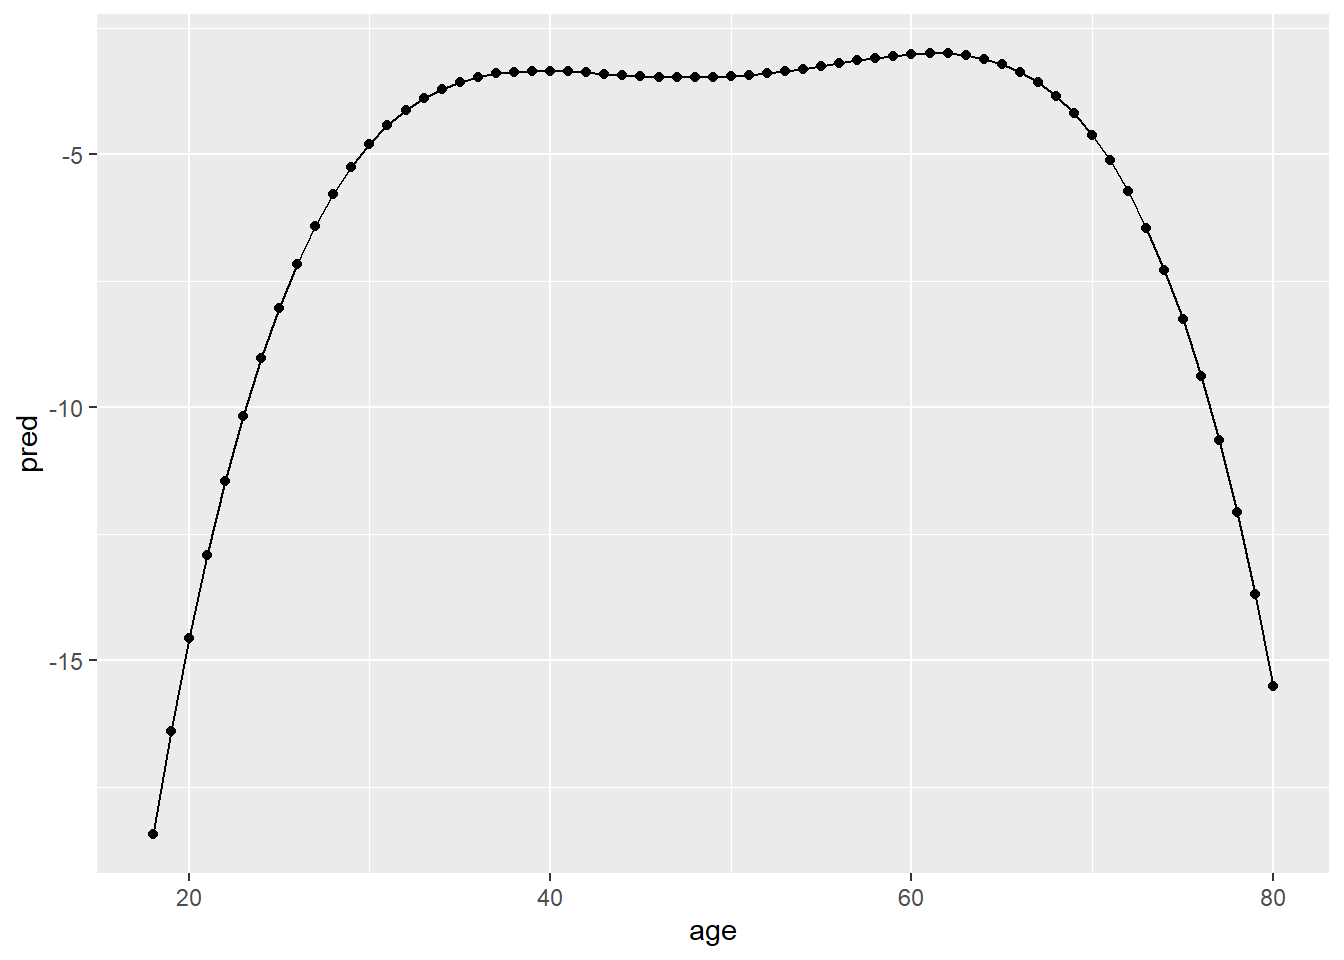
\includegraphics{notes_islr6_files/figure-latex/unnamed-chunk-4-1.pdf}

\begin{Shaded}
\begin{Highlighting}[]
\NormalTok{eigens <-}\StringTok{ }\KeywordTok{as.matrix}\NormalTok{(dat[,}\DecValTok{1}\OperatorTok{:}\DecValTok{2}\NormalTok{]) }\OperatorTok\StringTok{ }\NormalTok{eigens}\OperatorTok{$}\NormalTok{vectors}
\KeywordTok{dimnames}\NormalTok{(eigens) <-}\StringTok{ }\NormalTok{NULL}\CommentTok{#\{map2_dfr(as.data.frame(.$vectors), .$values, `*`)\}}

\KeywordTok{cbind}\NormalTok{(dat[,}\DecValTok{1}\OperatorTok{:}\DecValTok{2}\NormalTok{], eigens }\OperatorTok\StringTok{ }\NormalTok{t) }\OperatorTok\StringTok{ }
\StringTok{  }\KeywordTok{ggplot}\NormalTok{(}\KeywordTok{aes}\NormalTok{(}\DataTypeTok{x =}\NormalTok{ wt, }\DataTypeTok{y =}\NormalTok{ mpg)) }\OperatorTok{+}
\StringTok{  }\KeywordTok{geom_point}\NormalTok{() }\OperatorTok{+}
\StringTok{  }\KeywordTok{geom_segment}\NormalTok{(}\KeywordTok{aes}\NormalTok{(}\DataTypeTok{xend =} \DecValTok{0}\NormalTok{, }\DataTypeTok{yend =} \DecValTok{0}\NormalTok{))}\OperatorTok{+}
\StringTok{  }\KeywordTok{scale_color_manual}\NormalTok{(}\DataTypeTok{values =} \KeywordTok{c}\NormalTok{( }\DataTypeTok{x =}\StringTok{"red"}\NormalTok{, }\DataTypeTok{y =}\StringTok{"green"}\NormalTok{)) }\OperatorTok{+}
\StringTok{  }\KeywordTok{geom_point}\NormalTok{(}\KeywordTok{aes}\NormalTok{(}\DataTypeTok{x =} \StringTok{`}\DataTypeTok{1}\StringTok{`}\NormalTok{, }\DataTypeTok{y =} \StringTok{`}\DataTypeTok{2}\StringTok{`}\NormalTok{))}\OperatorTok{+}
\StringTok{  }\KeywordTok{geom_segment}\NormalTok{(}\KeywordTok{aes}\NormalTok{(}\DataTypeTok{x =}\StringTok{`}\DataTypeTok{1}\StringTok{`}\NormalTok{, }\DataTypeTok{y =} \StringTok{`}\DataTypeTok{2}\StringTok{`}\NormalTok{, }\DataTypeTok{xend =} \DecValTok{0}\NormalTok{, }\DataTypeTok{yend =}\DecValTok{0}\NormalTok{), }\DataTypeTok{col =} \StringTok{"blue"}\NormalTok{) }\OperatorTok{+}
\StringTok{  }\KeywordTok{xlim}\NormalTok{(}\KeywordTok{c}\NormalTok{(}\OperatorTok{-}\FloatTok{1.5}\NormalTok{,}\FloatTok{1.5}\NormalTok{)) }\OperatorTok{+}
\StringTok{  }\KeywordTok{ylim}\NormalTok{(}\KeywordTok{c}\NormalTok{(}\OperatorTok{-}\FloatTok{1.5}\NormalTok{,}\FloatTok{1.5}\NormalTok{)) }\OperatorTok{+}
\StringTok{  }\KeywordTok{geom_vline}\NormalTok{(}\DataTypeTok{xintercept =} \DecValTok{0}\NormalTok{) }\OperatorTok{+}
\StringTok{  }\KeywordTok{geom_hline}\NormalTok{(}\DataTypeTok{yintercept =} \DecValTok{0}\NormalTok{) }\OperatorTok{+}
\StringTok{  }\KeywordTok{geom_segment}\NormalTok{(}\KeywordTok{aes}\NormalTok{(}\DataTypeTok{xend =}\DecValTok{0}\NormalTok{, }\DataTypeTok{yend =} \DecValTok{0}\NormalTok{, }\DataTypeTok{x =} \DecValTok{0}\NormalTok{, }\DataTypeTok{y =} \DecValTok{1}\NormalTok{), }\DataTypeTok{col =} \StringTok{"green"}\NormalTok{) }\OperatorTok{+}
\StringTok{  }\KeywordTok{geom_segment}\NormalTok{(}\KeywordTok{aes}\NormalTok{(}\DataTypeTok{xend =}\DecValTok{0}\NormalTok{, }\DataTypeTok{yend =} \DecValTok{0}\NormalTok{, }\DataTypeTok{x =} \DecValTok{1}\NormalTok{, }\DataTypeTok{y =} \DecValTok{0}\NormalTok{), }\DataTypeTok{col =} \StringTok{"red"}\NormalTok{) }\OperatorTok{+}
\StringTok{  }\KeywordTok{labs}\NormalTok{(}\DataTypeTok{title =} \StringTok{"Eigenvectors after Matrix Transformation"}\NormalTok{)}
\end{Highlighting}
\end{Shaded}

\includegraphics{notes_islr6_files/figure-latex/unnamed-chunk-4-2.pdf}

The eigenvectors of the covariance or correlation matrix give these
directions of maximal variance. (Note \(\frac{X^TX}{n-1}\) gives the
covariance matrix). The correlation/covaraince matrix itself really
expresses the data with an alternate basis giving relative
relationships, compressing or elongating the basis vectors in the
directions of most variance. If data are plotted after transformation by
the cor/cov matrix, they will cluster along the eignvectors - the axes
of the transformation, where varaince is maximal. All are orthogonal to
each other, maximizing variance captured when projecting data onto the
eigenvectors. Constructing components involves taking the desired number
of eigenvectors and multiplying the scaled data by the egienvectors
matrix; each component is the matrix-vector product of the data matrix
and an eigenvector. A single element of component vector \(j\) is
\[y = zv^T\], where v is an element of a column of the eigens matrix.
Additional components can be found by subtracting the first component
from \(X\) and then finding the weight vector that maximizes captured
variance. It turns out this is always the eigenvector with the
next-highest eigenvalue. From another standpoint, each additional
component explains as much as possible of the error produced by the
previous one. The equation to project the data onto the components is:

\[Y = V^TZ^T\] or \[Y = (ZT)^T\], where \(V\) is a \(p\times p\)
(or\(p\times{m}\), if \(m\) eigenvectors are chosen) eigenvector matrix
that transforms each standardized \(z_{ij}\) of Z into a reproduction of
the response. This is equivalent to translating the data to a coordinate
system where each component forms the axis of a dimension. This works
for any number of components, since \(Z\) has as many columns as each
eigenvector has rows. Maximizing variance means maximizing \(X^TX\)
(i.e., squared distances). This is a positive semidefinite
matrix(\(z^tMz\) is positive or zero for all real \(z\)). The first
eigenvector gives the maximum quantity for such a matrix.

To project the whole data on tho the components (a \(n\timesp\) matrix),
compute \(Z*=ZV\), using the full eigens matrix. This gives the
transpose of the \(Y\) defined above

Illustration:

\begin{Shaded}
\begin{Highlighting}[]
\KeywordTok{tibble}\NormalTok{(}\DataTypeTok{PC1=}\OperatorTok{-}\DecValTok{20}\OperatorTok{:}\DecValTok{20}\NormalTok{, }\DataTypeTok{PC2=}\KeywordTok{rnorm}\NormalTok{(}\DataTypeTok{mean =} \DecValTok{0}\NormalTok{, }\DataTypeTok{sd =} \DecValTok{5}\NormalTok{, }\DataTypeTok{n =} \DecValTok{41}\NormalTok{)) }\OperatorTok\StringTok{ }
\StringTok{  }\KeywordTok{ggplot}\NormalTok{(}\KeywordTok{aes}\NormalTok{(}\DataTypeTok{x =}\NormalTok{ PC1, }\DataTypeTok{y =}\NormalTok{ PC2)) }\OperatorTok{+}
\StringTok{  }\KeywordTok{geom_point}\NormalTok{()}\OperatorTok{+}
\StringTok{  }\KeywordTok{geom_hline}\NormalTok{(}\DataTypeTok{yintercept =} \DecValTok{0}\NormalTok{) }\OperatorTok{+}
\StringTok{  }\KeywordTok{scale_y_continuous}\NormalTok{(}\DataTypeTok{limits =} \KeywordTok{c}\NormalTok{(}\OperatorTok{-}\DecValTok{10}\NormalTok{, }\DecValTok{10}\NormalTok{)) }\OperatorTok{+}
\StringTok{  }\KeywordTok{geom_segment}\NormalTok{(}\KeywordTok{aes}\NormalTok{(}\DataTypeTok{x =}\NormalTok{ PC1, }\DataTypeTok{xend =}\NormalTok{ PC1, }\DataTypeTok{y =} \DecValTok{0}\NormalTok{, }\DataTypeTok{yend =}\NormalTok{ PC2), }\DataTypeTok{linetype =} \StringTok{"dashed"}\NormalTok{) }\OperatorTok{+}
\StringTok{  }\KeywordTok{geom_point}\NormalTok{(}\KeywordTok{aes}\NormalTok{(}\DataTypeTok{y =} \DecValTok{0}\NormalTok{), }\DataTypeTok{shape =} \DecValTok{4}\NormalTok{)}\OperatorTok{+}
\StringTok{  }\KeywordTok{geom_vline}\NormalTok{(}\KeywordTok{aes}\NormalTok{(}\DataTypeTok{xintercept =} \DecValTok{0}\NormalTok{))}
\end{Highlighting}
\end{Shaded}

\begin{verbatim}
## Warning: Removed 2 rows containing missing values (geom_point).
\end{verbatim}

\begin{verbatim}
## Warning: Removed 2 rows containing missing values (geom_segment).
\end{verbatim}

\includegraphics{notes_islr6_files/figure-latex/unnamed-chunk-5-1.pdf}

For the example given above, each value of the first PC can be seen as a
one-number summary of the scores of pop and ad for that observation. A
negative score indicates below-average values for each (since each
loading is positive). The first PC is poistively correlated with each
predictor. Since the second PC must be orthogonal (simply perprendicular
in 2D space), the loadings are .0544 and -.0839 (the sign of ad's
loading second reversed). This component has lower scores, indicating it
captures less information. It has weaker correlation with either
predictor. It is easy to see from the plot that a second component
perpendicular to the first completely decribes the position of each
point, since there are just two predictors.

Geometrically, once the data are projected onto the first component,
each subsequent component is fitted on the resideuals (the variance
unexplained by the projection), which is why they are orthogonal.
Together, the components form an alternate coordinate system.

The main benefit of all this is it saves us from estimating
\[\frac{p(p-1)}{p}\] parameters for a full model, largely the
covariances.

\hypertarget{principal-components-regression}{%
\subsubsection{Principal Components
Regression}\label{principal-components-regression}}

PCR assumes that the directions of most variation in \(X\) - the
components - are those associated with \(Y\). By capturing only relevant
variacne, we can get a better model than a standard OLS fit. Adding
components reduces bias but increases variance (of course), giving the
typical U curve for MSE. PCR does well comapred to the lasso and RR if
only a few PC are necessary and poorly if many are required. Components
are also not easily interpretable.

PCR is not truly a feature selection method, since each PC is a linear
combination of every predictor. The number of components is usually
chosen by cross-validation. As with RR, standardizing is crucial to
prevent some predictors from having too much impact.

\hypertarget{excess-detail-why-is-it-eigenvectors}{%
\subsubsection{Excess Detail: Why Is It
Eigenvectors?}\label{excess-detail-why-is-it-eigenvectors}}

\url{https://stats.stackexchange.com/questions/217995/what-is-an-intuitive-explanation-for-how-pca-turns-from-a-geometric-problem-wit}

Any square matrix can be decomposed as \(A=PDP^-1\), where \(P\) is the
eigenvectors matrix and \(D\) is the diagonal matrix of the eigenvalues
(each eigen on the trace, zeroes otherwise). This works because
\(Av=\lambda{v}\). Scaling the eigenvector inverse by the
egeinvectvalues, \emph{scalars which for the eigenvectors represent the
effect of the matrix transformation}, yields a matrix which yields the
original matrix when multiplied by the eigenvectors, instead of just the
identity (the usual product of matrix and inverse).

\begin{Shaded}
\begin{Highlighting}[]
\NormalTok{example <-}\StringTok{ }\KeywordTok{cor}\NormalTok{(mtcars)}
\NormalTok{example}
\end{Highlighting}
\end{Shaded}

\begin{verbatim}
##             mpg        cyl       disp         hp        drat         wt
## mpg   1.0000000 -0.8521620 -0.8475514 -0.7761684  0.68117191 -0.8676594
## cyl  -0.8521620  1.0000000  0.9020329  0.8324475 -0.69993811  0.7824958
## disp -0.8475514  0.9020329  1.0000000  0.7909486 -0.71021393  0.8879799
## hp   -0.7761684  0.8324475  0.7909486  1.0000000 -0.44875912  0.6587479
## drat  0.6811719 -0.6999381 -0.7102139 -0.4487591  1.00000000 -0.7124406
## wt   -0.8676594  0.7824958  0.8879799  0.6587479 -0.71244065  1.0000000
## qsec  0.4186840 -0.5912421 -0.4336979 -0.7082234  0.09120476 -0.1747159
## vs    0.6640389 -0.8108118 -0.7104159 -0.7230967  0.44027846 -0.5549157
## am    0.5998324 -0.5226070 -0.5912270 -0.2432043  0.71271113 -0.6924953
## gear  0.4802848 -0.4926866 -0.5555692 -0.1257043  0.69961013 -0.5832870
## carb -0.5509251  0.5269883  0.3949769  0.7498125 -0.09078980  0.4276059
##             qsec         vs          am       gear        carb
## mpg   0.41868403  0.6640389  0.59983243  0.4802848 -0.55092507
## cyl  -0.59124207 -0.8108118 -0.52260705 -0.4926866  0.52698829
## disp -0.43369788 -0.7104159 -0.59122704 -0.5555692  0.39497686
## hp   -0.70822339 -0.7230967 -0.24320426 -0.1257043  0.74981247
## drat  0.09120476  0.4402785  0.71271113  0.6996101 -0.09078980
## wt   -0.17471588 -0.5549157 -0.69249526 -0.5832870  0.42760594
## qsec  1.00000000  0.7445354 -0.22986086 -0.2126822 -0.65624923
## vs    0.74453544  1.0000000  0.16834512  0.2060233 -0.56960714
## am   -0.22986086  0.1683451  1.00000000  0.7940588  0.05753435
## gear -0.21268223  0.2060233  0.79405876  1.0000000  0.27407284
## carb -0.65624923 -0.5696071  0.05753435  0.2740728  1.00000000
\end{verbatim}

\begin{Shaded}
\begin{Highlighting}[]
\KeywordTok{eigen}\NormalTok{(example)}\OperatorTok{$}\NormalTok{vectors }\OperatorTok\StringTok{ }\KeywordTok{diag}\NormalTok{(}\KeywordTok{eigen}\NormalTok{(example)}\OperatorTok{$}\NormalTok{values) }\OperatorTok\StringTok{ }\KeywordTok{solve}\NormalTok{(}\KeywordTok{eigen}\NormalTok{(example)}\OperatorTok{$}\NormalTok{vectors)}
\end{Highlighting}
\end{Shaded}

\begin{verbatim}
##             [,1]       [,2]       [,3]       [,4]        [,5]       [,6]
##  [1,]  1.0000000 -0.8521620 -0.8475514 -0.7761684  0.68117191 -0.8676594
##  [2,] -0.8521620  1.0000000  0.9020329  0.8324475 -0.69993811  0.7824958
##  [3,] -0.8475514  0.9020329  1.0000000  0.7909486 -0.71021393  0.8879799
##  [4,] -0.7761684  0.8324475  0.7909486  1.0000000 -0.44875912  0.6587479
##  [5,]  0.6811719 -0.6999381 -0.7102139 -0.4487591  1.00000000 -0.7124406
##  [6,] -0.8676594  0.7824958  0.8879799  0.6587479 -0.71244065  1.0000000
##  [7,]  0.4186840 -0.5912421 -0.4336979 -0.7082234  0.09120476 -0.1747159
##  [8,]  0.6640389 -0.8108118 -0.7104159 -0.7230967  0.44027846 -0.5549157
##  [9,]  0.5998324 -0.5226070 -0.5912270 -0.2432043  0.71271113 -0.6924953
## [10,]  0.4802848 -0.4926866 -0.5555692 -0.1257043  0.69961013 -0.5832870
## [11,] -0.5509251  0.5269883  0.3949769  0.7498125 -0.09078980  0.4276059
##              [,7]       [,8]        [,9]      [,10]       [,11]
##  [1,]  0.41868403  0.6640389  0.59983243  0.4802848 -0.55092507
##  [2,] -0.59124207 -0.8108118 -0.52260705 -0.4926866  0.52698829
##  [3,] -0.43369788 -0.7104159 -0.59122704 -0.5555692  0.39497686
##  [4,] -0.70822339 -0.7230967 -0.24320426 -0.1257043  0.74981247
##  [5,]  0.09120476  0.4402785  0.71271113  0.6996101 -0.09078980
##  [6,] -0.17471588 -0.5549157 -0.69249526 -0.5832870  0.42760594
##  [7,]  1.00000000  0.7445354 -0.22986086 -0.2126822 -0.65624923
##  [8,]  0.74453544  1.0000000  0.16834512  0.2060233 -0.56960714
##  [9,] -0.22986086  0.1683451  1.00000000  0.7940588  0.05753435
## [10,] -0.21268223  0.2060233  0.79405876  1.0000000  0.27407284
## [11,] -0.65624923 -0.5696071  0.05753435  0.2740728  1.00000000
\end{verbatim}

PCA seeks to project data onto whichever direction has the highest
variance of the new coordinates. If \(C\) is the covaraince matrix, we
want a 1-length vector \(w\) (\(w^Tw=1\)) such that the scalareigen)
\(w^TCw\) is as high as possible. \(w\) must be unit-length
(\(\mid\midw\mid\mid=1\)) because making it longer would allow us to
make the expression infinite. (We use the transpose becuase variance
involves squared distances). This projection would be \(Xw\) with
variance \(\frac{n}{n-1}(Xw)^T\cdot{Xw}\).

The usual explantation involves adding a Lagrange multiplier and
differentitating, which gives the eigenvector equation. Substituting
into the maximization function gives \(\lambda\); since we are
maximizing, we want the eigenvector with the highest eigenvalue.

Eigendecomposition is easier to follow. With he eigendecomposition,
\(w^TCw\) can be rewritten \(\sum{w^2_i}\lambda_i\) (each element of
\(w\) squared and scaled by the eigenvalue). Here the \(w_i\) are
eigenvectors. Clearly, this is maximized if \(w = (1,0,0,\dots,0)\) -
that is, the first eigenvector, giving variance \(\lambda_1\).

This follows from the spectral theorem. Assume the first eigenvector of
the symmetric matrix \(C\), \(w_1\) replaces the first basis vector
(such that \(w_1 = (1,0,0...0)\). In other words, we substitute the
first eigenvector for \(\hat{i}\). Writing a matrix in this form, every
element represents its distance from the corresponding element of the
eigenvector, as elements in matrices in standard form represent
distances from the corresponding elements of basis vectors. Any matrix
is really a linear combination of basis vectors scaled by varying
quantities. PCR software outputs the values of the eigenvectors in the
\emph{original} coordinate system. The first element of \(C\)'s trace
becomes \(\lambda_1\), because
\(Cw_1=\lambda_1w_1 = (\lambda_1,0,0,0...0)\) - i.e., by definition,
multiplying the first column of \(C\) by the eigenvector is the same as
scaling the eigenvector by its eigenvalue. In other words, the matrix is
decomposed as a linear combiantion of basis eigenvectors and eigenvalue
scalars. The matrix is symmetric. So C becomes: \[C =
\begin{pmatrix}
\lambda_1&0&\dots&0\\
0\\
.\\
.\\
.\\
0
\end{pmatrix}\] (remmebr this is just the identity multiplied by the
diagonal eigenvalue matrix).

Equivalently, each eigenvector can be seen as a 1D subspace where \(C\)
behaves like the scalar \(\lambda_i\)

The whole matrix can be filled in by repeating the same algorithm
(eigenvector replacing each basis vector, with \(\lambda_i\) on the
trace) for each block, since it is symmetric.

Given the unit-length constraint, \(w^TCw\) is obviously maximized with
basis vectors for \(w\) - \(w= (1,0,0...0)\), etc. In the eigenbasis,
these equate to the diagonal matrix of eigenvalues. Therefore, each
eigenvalue gives the maximum varaince that can be extracted by a single
\(w\),a nd the corresponding \(w_p\) are the eigenvectors of \(C\).

\hypertarget{partial-least-squares}{%
\subsubsection{Partial Least Squares}\label{partial-least-squares}}

PCR is unsupervised - the response \(Y\) plays no role in selecting the
components. Partial least squares differs from PCR in this respect.
After standardization, each loading \(\phi_j1\) is obtained from
\(\beta_j\) of a regression of \(Y\) onto \(X_j\). So each loading
represents the average change of the response in response to that
predictor alone, no eigens involved. These coffeicients are proportional
to correlations, so the predictors most closely related to the response
receive higher loadings. To find additional directions, we regress each
variable on \(Z_1\) (the first component) and take the residuals. These
represent variation unexplained by the first componenet. We then regress
each predictor on each set of residuals and obtain \(Z_2\) the same way
as \(Z_1\). Once all loadings are obtained, the model is fit in the same
fashion as PCR.

Overall, supervision increases variance relative to PCR but reduces
bias.

\hypertarget{considerations-for-higher-dimensions}{%
\section{COnsiderations for Higher
Dimensions}\label{considerations-for-higher-dimensions}}

Traditonal regression techniques struggle for high-dimensional settings,
increasingly common with enhanced data collection, with hundreds of
mesaurements for each observation. When \(p >n\), OLS gives a perfect
fit of no use in predicting test data. There is no unique solution
because the predictors matrix spans the dimesnion of the response
vector; the response can be perfectly reproduced by many linear
combinations of \(X\). Intutiively, a straigt line can connect all the
points with no redisual. In other words, unmodified OLS is too flexible.
This holds true even if the predictors are totally unrelated to the
response. However, adding more predicors hugely increases test MSE by
increasing variance.

\(C_p\), the BIC, and the AIC are of little help becuase
\(\hat\sigma^2\) cannot be reliably estimated with very many predictors.
The methods discussed above address these problems by reducing the
flexibility of linear modeling by shirnking or eliminating parameters.
The lasso, for instance, has degrees of freedom equal to the number of
nonzero coefs estimated.

This is the curse of dimensionality: additional features improve the fit
only if truly assoicated with the response.

In this stupid model, there are no degrees of freedom, so no residuals
whatsoever.

\begin{Shaded}
\begin{Highlighting}[]
\NormalTok{dat <-}\StringTok{ }\KeywordTok{replicate}\NormalTok{(}\DecValTok{100}\NormalTok{, }\KeywordTok{sample}\NormalTok{(}\OperatorTok{-}\NormalTok{(}\DecValTok{10}\OperatorTok{^}\DecValTok{4}\NormalTok{)}\OperatorTok{:}\DecValTok{10}\OperatorTok{^}\DecValTok{4}\NormalTok{, }\DecValTok{10}\NormalTok{, }\DataTypeTok{replace =}\NormalTok{ T)) }\OperatorTok\StringTok{ }\KeywordTok{as.matrix}\NormalTok{() }\OperatorTok\StringTok{ }\KeywordTok{cbind}\NormalTok{(., }\DataTypeTok{y =} \KeywordTok{rnorm}\NormalTok{(}\DecValTok{10}\NormalTok{) }\OperatorTok{+}\StringTok{ }\DecValTok{2}\NormalTok{) }\OperatorTok\StringTok{ }
\StringTok{  }\KeywordTok{as.data.frame}\NormalTok{()}
\NormalTok{dat }\OperatorTok\StringTok{ }\KeywordTok{lm}\NormalTok{(}\DataTypeTok{data =}\NormalTok{., y }\OperatorTok{~}\NormalTok{.) }\OperatorTok\StringTok{ }\NormalTok{summary}
\end{Highlighting}
\end{Shaded}

\begin{verbatim}
## 
## Call:
## lm(formula = y ~ ., data = .)
## 
## Residuals:
## ALL 10 residuals are 0: no residual degrees of freedom!
## 
## Coefficients: (91 not defined because of singularities)
##               Estimate Std. Error t value Pr(>|t|)
## (Intercept)  1.185e+00         NA      NA       NA
## V1           1.878e-04         NA      NA       NA
## V2           1.591e-04         NA      NA       NA
## V3           1.208e-04         NA      NA       NA
## V4           7.997e-05         NA      NA       NA
## V5          -8.993e-05         NA      NA       NA
## V6          -8.423e-05         NA      NA       NA
## V7           7.060e-05         NA      NA       NA
## V8          -1.545e-04         NA      NA       NA
## V9           1.924e-05         NA      NA       NA
## V10                 NA         NA      NA       NA
## V11                 NA         NA      NA       NA
## V12                 NA         NA      NA       NA
## V13                 NA         NA      NA       NA
## V14                 NA         NA      NA       NA
## V15                 NA         NA      NA       NA
## V16                 NA         NA      NA       NA
## V17                 NA         NA      NA       NA
## V18                 NA         NA      NA       NA
## V19                 NA         NA      NA       NA
## V20                 NA         NA      NA       NA
## V21                 NA         NA      NA       NA
## V22                 NA         NA      NA       NA
## V23                 NA         NA      NA       NA
## V24                 NA         NA      NA       NA
## V25                 NA         NA      NA       NA
## V26                 NA         NA      NA       NA
## V27                 NA         NA      NA       NA
## V28                 NA         NA      NA       NA
## V29                 NA         NA      NA       NA
## V30                 NA         NA      NA       NA
## V31                 NA         NA      NA       NA
## V32                 NA         NA      NA       NA
## V33                 NA         NA      NA       NA
## V34                 NA         NA      NA       NA
## V35                 NA         NA      NA       NA
## V36                 NA         NA      NA       NA
## V37                 NA         NA      NA       NA
## V38                 NA         NA      NA       NA
## V39                 NA         NA      NA       NA
## V40                 NA         NA      NA       NA
## V41                 NA         NA      NA       NA
## V42                 NA         NA      NA       NA
## V43                 NA         NA      NA       NA
## V44                 NA         NA      NA       NA
## V45                 NA         NA      NA       NA
## V46                 NA         NA      NA       NA
## V47                 NA         NA      NA       NA
## V48                 NA         NA      NA       NA
## V49                 NA         NA      NA       NA
## V50                 NA         NA      NA       NA
## V51                 NA         NA      NA       NA
## V52                 NA         NA      NA       NA
## V53                 NA         NA      NA       NA
## V54                 NA         NA      NA       NA
## V55                 NA         NA      NA       NA
## V56                 NA         NA      NA       NA
## V57                 NA         NA      NA       NA
## V58                 NA         NA      NA       NA
## V59                 NA         NA      NA       NA
## V60                 NA         NA      NA       NA
## V61                 NA         NA      NA       NA
## V62                 NA         NA      NA       NA
## V63                 NA         NA      NA       NA
## V64                 NA         NA      NA       NA
## V65                 NA         NA      NA       NA
## V66                 NA         NA      NA       NA
## V67                 NA         NA      NA       NA
## V68                 NA         NA      NA       NA
## V69                 NA         NA      NA       NA
## V70                 NA         NA      NA       NA
## V71                 NA         NA      NA       NA
## V72                 NA         NA      NA       NA
## V73                 NA         NA      NA       NA
## V74                 NA         NA      NA       NA
## V75                 NA         NA      NA       NA
## V76                 NA         NA      NA       NA
## V77                 NA         NA      NA       NA
## V78                 NA         NA      NA       NA
## V79                 NA         NA      NA       NA
## V80                 NA         NA      NA       NA
## V81                 NA         NA      NA       NA
## V82                 NA         NA      NA       NA
## V83                 NA         NA      NA       NA
## V84                 NA         NA      NA       NA
## V85                 NA         NA      NA       NA
## V86                 NA         NA      NA       NA
## V87                 NA         NA      NA       NA
## V88                 NA         NA      NA       NA
## V89                 NA         NA      NA       NA
## V90                 NA         NA      NA       NA
## V91                 NA         NA      NA       NA
## V92                 NA         NA      NA       NA
## V93                 NA         NA      NA       NA
## V94                 NA         NA      NA       NA
## V95                 NA         NA      NA       NA
## V96                 NA         NA      NA       NA
## V97                 NA         NA      NA       NA
## V98                 NA         NA      NA       NA
## V99                 NA         NA      NA       NA
## V100                NA         NA      NA       NA
## 
## Residual standard error: NaN on 0 degrees of freedom
## Multiple R-squared:      1,  Adjusted R-squared:    NaN 
## F-statistic:   NaN on 9 and 0 DF,  p-value: NA
\end{verbatim}

\hypertarget{interpreting-results-in-high-dimensions}{%
\subsubsection{Interpreting Results in High
Dimensions}\label{interpreting-results-in-high-dimensions}}

High-deimensioanl settings are highly multicollinear - any predictor can
be expressed as alinear combination of the others. It follows that we
cannot isolate any predictors as truly influential, nor find optiaml
regression coefficients. Each good-fitting model is only one of many
possibilites. Additionally, training set measurements like \(R^2\) 2are
useless for predicting performance on high-dimensional data.

\end{document}
